\documentclass[11pt]{article}
%\usepackage{uvatoc} % replace this line with the one below for your submission
\usepackage[response]{uvatoc}



\begin{document}

\makeheader

\makemytitle{Week 6: Automata Tune}

\submitter {Benjamin (aqn9yv, dlb2ru, ht6xd, iad4de, jmn4fms, lw7jz)}

\directions{
\collaboration{You should work on the problems yourself, before discussing with
others, and with your cohorts are your cohort meeting. By the Assessed Cohort Meeting,
you and all of your cohortmates, should be prepared to present and discuss solutions to
all of the assigned problems (including the programming problems). In addition to discussing with your cohortmates, you may
discuss the problems with anyone you want, and use any resources you want except for
any materials from previous offerings of this course, which are not permitted.}
}

\begin{definition}
Define L to be the language computed by $M = (Q, \Sigma, \delta, q_{0}, F)$
\end{definition}

\begin{problem}
Infinite Languages
\end{problem}
\directions{
Show that the language computed by a finite state automaton is infinite if and only if there is some string accepted by the automaton with more characters than the automaton has states. That is, show that for finite state automaton $M=(Q, \Sigma, \delta, q_0, F)$ the size of the language computed by $M$ is infinite if and only if there is some $s\in \Sigma^*$ such that $|s| >|Q|$.
}

\newtheorem{theorem}{Theorem}

\begin{theorem}

(Formatting the theorem in logical language)
\begin{equation}
    |L| = \infty \iff \exists s \in \Sigma^* . \; |s| > |Q|
\end{equation}

\end{theorem}

\begin{proof}

\paragraph{Forward Direction}

We want to show that if $|L|$ is infinite, then $\exists s\in \Sigma^* $ such that  $|s| > |Q|$. We proceed by contradiction.

Assume, for the sake of contradiction, $\neg (\exists s \in \Sigma^* $ such that  $|s| > |Q|)$. This is equivalent to $\forall s \in \Sigma^*, |s| \leq |Q|$. 

$\implies$ There are at most ${|s|}^{|Q|}$ possible combination of characters in $\Sigma^*$.

$\implies$ The number of strings accepted by the language is a subset of ${\Sigma}^{*}$ by definition, and so $|L| \leq |\Sigma^*|$ $\leq$ ${|s|}^{|Q|}$

$\implies$ The number of strings in L is finite. This contradicts what we know to be true, that $|L|$ is infinite. (since we are proving for the forward direction)

$\implies$ Our assumption must be false, so $\exists s\in \Sigma^* $ such that  $|s|  > |Q|$.

\paragraph{Backward Direction}

If $\exists s\in \Sigma^* $ such that $|s| > |Q|$, then $|L|$ is infinite. Let $n = |Q|$.

First we will show that for some $i,j \in \mathbb{Z}$ such that $i \neq j$ we have that $\delta^{i}[(q_{0},s)] = \delta^{j}[(q_{0},s)]$.

Assume that for the first $n$ bits in s, $b_{0}, ... , b_{n}$, that each state, $q_{0},..., q_{n}$, is transitioned to only once. Then the next ($|s|-n$) bits of s must transition either back to their current state, or to a previous state.

If that assumption is false, then we get for free that there is some state transitioned to more than once in the first $n$ bits of s.

In either case, we have that for some $i,j \in \mathbb{Z}$ s.t. $i \neq j$, $\delta^{i}[(q_{0},s)] = \delta^{j}[(q_{0},s)]$.

We can assume without loss of generality that $i < j$, and let $k = a*(j-i)+r$, for any $a\in \N$ where $|s| = j + r$. Then let $s'$ be another string with the same first $i$ bits of $s$, and the same final $r$ bits of s. Let the middling $a*(j-i)$ bits of $s'$ be $a$ repetitions of the $i^{th}$ through the $j^{th}$ bits of $s$.

$\implies$ computing $\delta^{i+k}[(q_0,s')]$ is equivalent to $\delta^{r}[(\delta^{i}(q_0,s),s')]$.

Intuitively this is the same as noting that the FSA evaluating the bitstring s contains a loop. Let $q_{i}$ denote the state such that $q_{i} = \delta^{i}(q_{0},s)$, or simply the state after computing the first $i$ bits of s. Then computing the next $(j-i)$ bits of s returns simply returns us to $q_{i}$ by going around the loop.

What this means is we can construct another string $s'$ so that computing $s'$ arrives at state $q_{i}$ (i.e. the beginning of the loop), then traverses the loop $a$ times to return to $q_{i}$ again. The final $r$ bits of $s'$ are the same as $s$ so computing $s$ or $s'$ will end in the same state, call it $q_{F}$.

$\implies$ $a \in \mathbb{Z}$ has no upper bound, and so $k$ has no upper bound, therefore we can find an infinite number of k's satisfying $\delta^{i+k}[(q_0,s')]$ is equivalent to $\delta^{r}[(\delta^{i}(q_0,s),s')]$.

$\implies$ If we choose an initial $s \in \Sigma^*$ such that $|s| > |Q|$, which we know exists by assumption, and choose $s$ so that $q_{F}$ is $\in F$, then we can find an infinite number of strings $s'$ such that $s' \in L$ as well.

$\implies$ There are an infinite number of strings s' in the language.

Therefore $\exists s\in \Sigma^* $ such that $|s| > |Q|$ $\implies$ $|L| = \infty$.

\paragraph{Conclusion}
Thus we have proved both the forward direction and its converse, so

$\exists s\in \Sigma^* $ such that $|s| > |Q|$ $\iff$ $|L| = \infty$.

\paragraph{Alternatively, Cyclic Graph Proof of the Backward Direction}
% directed cyclic graph approach?

If there are more characters in an accepted string than the number of states in Q, and each input character to the FSA corresponds to an edge in the directed graph, then by the pigeonhole principle, at least one state must be visited twice after all characters of the string is accepted by the FSA.

This is only possible when there are at least one cycle in the graph of the FSA, so that some states could be visited more than once by walking along the cycle of the graph.

For example, in Figure 1 a cyclic FSA is given. The only way for the automata to accept an input string of length more than two is to have the string contain several substrings that walks either the loop of the state 0 (input "0" if current state is 0), or the loop of state 1 (input "1" if current state is 1), or the cycle between state 0 and state 1 (input "01" if current state is 1, or "10" if current is 0).

Since the input string contains substrings that loops the cycles of the graph, we can construct a new valid input string by repeatedly input the substring portion of the input string. For example, "010" is a valid input string for the FSA in Figure 1. We can construct a new valid input string by repeating the "10" substring as input, so that "01010" is also an input string. This process can be executed unlimited number of times, there are infinite number of valid strings that the FSA could take, meaning $|L| = \infty$.

\begin{figure}[ht!]
  \centering
  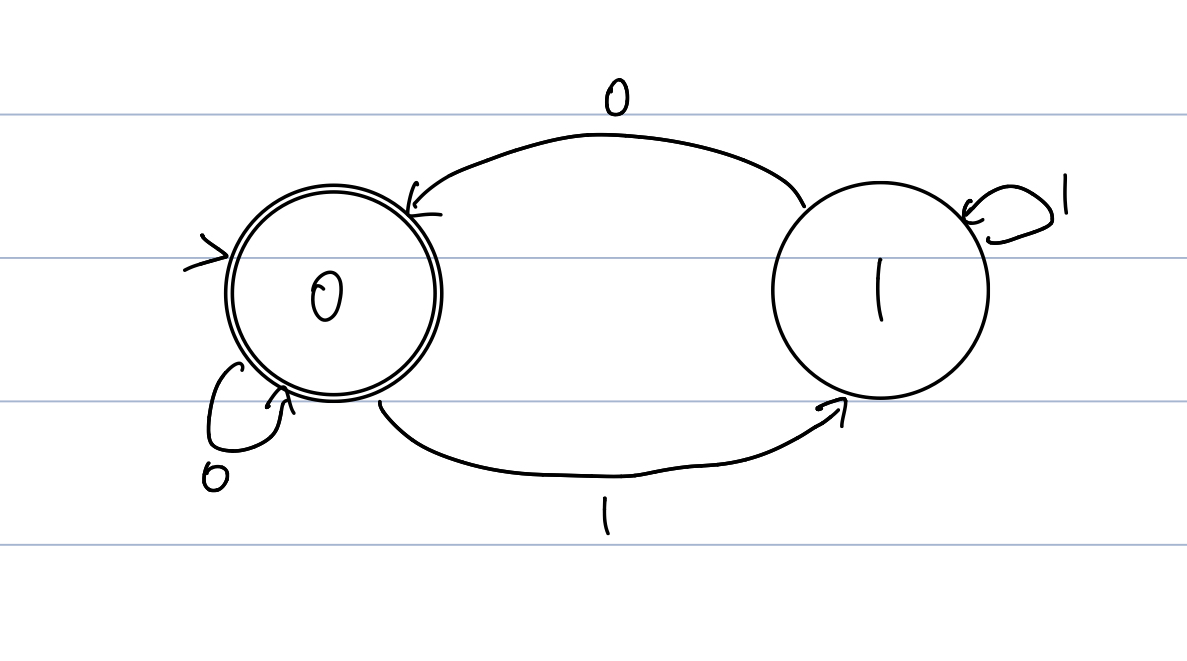
\includegraphics[origin = c, height = 30mm]{pic.jpeg}
  \caption{A Cyclic Finite State Automata}
\end{figure}

\end{proof}

\end{document}
